\chapter{Estudo de Campo}\label{cap:estudo-de-campo}

Este trabalho tem como seu principal objetivo desenvolver uma solução computacional que possibilite a melhoria
significativa da experiência dos usuários de transporte público da cidade de Picos. Para ser desenvolvido o projeto
foi dividido em três etapas, começando com uma pesquisa objetiva com os passageiros, com o propósito de entender
a realidade do problema que torna a utilização do transporte público insatisfatório.

Em uma pesquisa que contou com a participação de 87 pessoas que utilizam o transporte público em Picos, foi levantado os seguintes questionamentos:

\begin{lista}
\item Qual seu grau de satisfação com o transporte público de Picos?
\item Quando insatisfeito para quem você acha que pode e deve reclamar?
\item Quais os principais problemas enfrentados ao utilizar ônibus em Picos?
\item Qual sistema operacional do seu \textit{smartphone}?
\end{lista}

\begin{figure}[H]
\caption{Grau de Satisfação dos Usuários de Transporte Público de Picos}
\centering
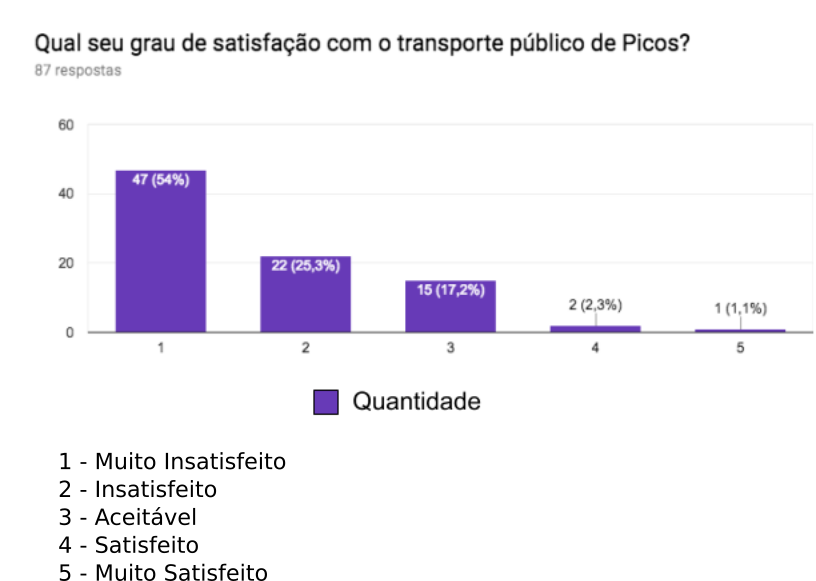
\includegraphics[width=.8\textwidth]{imagens/satisfacao.png}
\legend{Fonte: Autor}
\label{fig:satisfacao}
\end{figure}

O resultado obtido sobre a satisfação dos usuários pode ser visto na Figura \ref{fig:satisfacao}, onde foi determinado que escolhessem um valor pertencente ao intervalo de 1 a 5 para medir o grau de satisfação do usuário, onde o menor número representava o menor grau de satisfação possível, em que foi possível identificar que mais de 78\% dos usuários estão insatisfeitos com o transporte público, contudo também foi percebido que a maioria dos usuários não possuem uma forma de obter informações confiáveis e não tem conhecimento de onde podem fazer reclamações.

Ainda nessa mesma pesquisa foi possível identificar que os principais problemas encontrados foram o tempo de espera e as mudanças de horários dos ônibus sem aviso prévio da empresa prestadora do serviço.

\begin{figure}[H]
\caption{Gráfico dos Problemas Levantados do Transporte Público de Picos}
\centering
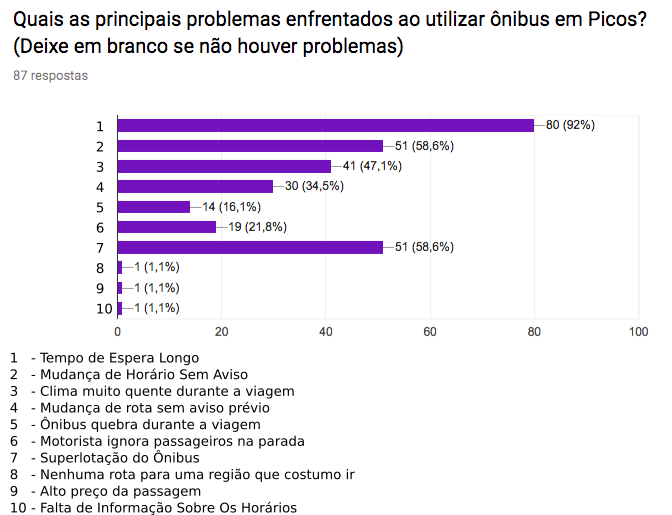
\includegraphics[width=1.0\textwidth]{imagens/problema.png}
\legend{Fonte: Autor}
\label{fig:problema}
\end{figure}

Na segunda etapa, mediante uma análise sobre os resultados da pesquisa com os passageiros e entrevistas realizadas com os fiscais e gestores do transporte público local, é nítido que a causa dos principais problemas é o fato dos usuários não terem acesso a informações sobre o funcionamento dos ônibus coletivos, tais como: horários, rotas e incidentes diários. Diante disso, constatou-se que para reduzir esses problemas é necessário desenvolver um meio de comunicação que forneça informações aos passageiros.

Ainda na segunda etapa é necessário que após a identificação e análise dos problemas seja determinado os requisitos para o desenvolvimento de um sistema computacional que auxilie na redução dos problemas identificados, entretanto, foi determinado previamente que a solução desenvolvida envolvesse o compartilhamento de dados em tempo real, como também a consulta dessas informações por meio de um aplicativo móvel.

\begin{figure}[H]
\caption{Gráfico Que Determina Onde os Passageiros Obtêm Informações}
\centering
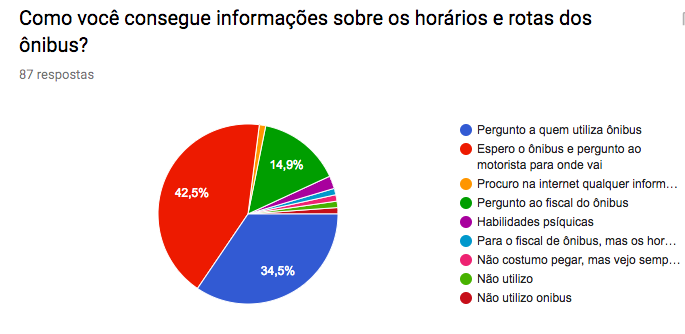
\includegraphics[width=1.0\textwidth]{imagens/informacao.png}
\legend{Fonte: Autor}
\label{fig:informacao}
\end{figure}

\begin{figure}[H]
\caption{Gráfico Que Determina Onde os Passageiros Efetuam Reclamação}
\centering
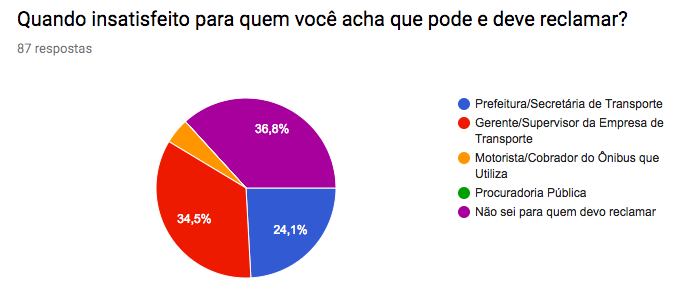
\includegraphics[width=1.0\textwidth]{imagens/reclamacao.png}
\legend{Fonte: Autor}
\label{fig:reclamacao}
\end{figure}

E na terceira e última etapa será aplicado uma metodologia de desenvolvimento ágil para a implementação dos softwares necessários para o funcionamento dos requisitos levantados na etapa 2, tal que, esse sistema será composto por um módulo de manutenção das informações providas ao usuário que será administrado pela empresa prestadora do serviço de transporte público e um módulo para consulta dessas informações pelos passageiros, como também serão implementadas funcionalidades que visam melhorar a comunicação direta entre os passageiros e os responsáveis pela prestação do serviço, por meio de formulários que permitam o passageiro efetuar reclamações e sugestões com a garantia de que os responsáveis recebam a mensagem, como também, permitir que as empresas enviem notificações para que todos os usuários tenham acesso rápido a informações que afetam diretamente a sua experiência de uso do transporte público urbano.